\documentclass{standalone}
\usepackage{tikz}

\begin{document}
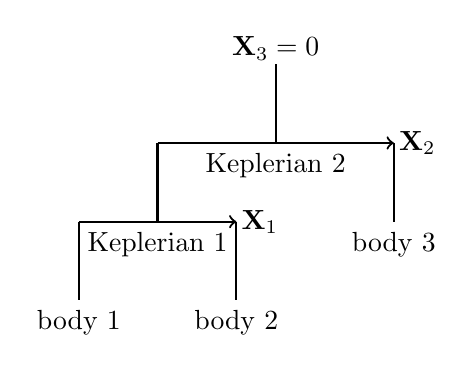
\begin{tikzpicture}

\draw[thick,->] (0,0) -- (3,0);
\draw[thick] (0,0) -- (0,-1) node[below] {Keplerian 1};
\draw[thick] (3,0) -- (3,-1) node[below] {body 3};
\draw[thick] (1.5,1) -- (1.5,0) node[below] {Keplerian 2};
\draw[thick,->] (-1,-1) -- (1,-1);
\draw[thick] (-1,-1) -- (-1,-2) node[below] {body 1};
\draw[thick] (1,-1) -- (1,-2) node[below] {body 2};
%\draw[thick,dashed,->] (0,0) -- (-2.,-2.8) node[below]{to observer at (0,0,-D)};
%\draw[->] (0,0) -- (2.2,0.5) node[right]{$(x,y,z)$};
%\draw[->] (2.2,0.5) -- (2.1,0.8) node[left]{$(\dot x,\dot y,\dot z)$};
\node[draw=none] at (1.3,-1) {$\mathbf{X}_1$};
\node[draw=none] at (3.3,0) {$\mathbf{X}_2$};
\node[draw=none] at (1.5,1.2) {$\mathbf{X}_3=0$};
\end{tikzpicture}

\end{document}
